\begin{center}
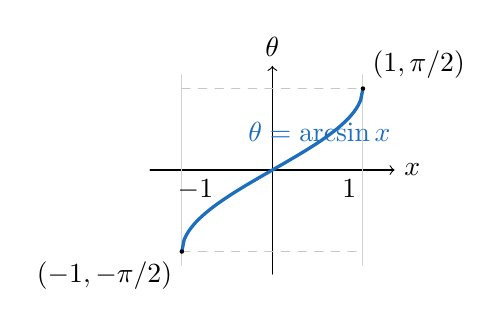
\begin{tikzpicture}[scale=1.15, line cap=round, line join=round]
  \definecolor{trigblue}{RGB}{30,110,190}
  \draw[->] (-1.35,0)--(1.35,0) node[right] {$x$};
  \draw[->] (0,-1.15)--(0,1.15) node[above] {$\theta$};
  \draw[gray!35] (-1,-1.05)--(-1,1.05);
  \draw[gray!35] (1,-1.05)--(1,1.05);
  \draw[gray!45,dashed] (-1,-0.9)--(1,-0.9);
  \draw[gray!45,dashed] (-1,0.9)--(1,0.9);
  \draw[very thick,trigblue,domain=-1:1,samples=80]
    plot ({\x},{0.9*asin(\x)/90});
  \fill (-1,-0.9) circle (0.025) node[below left] {$(-1,-\pi/2)$};
  \fill (1,0.9) circle (0.025) node[above right] {$(1,\pi/2)$};
  \node[trigblue] at (0.52,0.42) {$\theta=\arcsin x$};
  \node[below] at (0.85,0) {$1$};
  \node[below] at (-0.85,0) {$-1$};
\end{tikzpicture}
\end{center}
